\documentclass[conference]{IEEEtran}
\IEEEoverridecommandlockouts
% Based on the IEEE Conference Template (Overleaf): IEEEtran, conference mode.
\usepackage{cite}
\usepackage{amsmath,amssymb,amsfonts}
\usepackage{algorithmic}
\usepackage{algorithm}
\usepackage{graphicx}
\usepackage{textcomp}
\usepackage{xcolor}
\usepackage{booktabs}
\usepackage{multirow}
\usepackage{url}
\def\BibTeX{{\rm B\kern-.05em{\sc i\kern-.025em b}\kern-.08em
    T\kern-.1667em\lower.7ex\hbox{E}\kern-.125emX}}
\graphicspath{{figures/}}

\begin{document}

\title{False-Positive-Aware, Destination-Centric DDoS Detection and Source-Scoped Mitigation in Software-Defined Networks}

\author{
\IEEEauthorblockN{Advait Pathak}
\IEEEauthorblockA{\textit{Roll No. 23bcs094}}
\and
\IEEEauthorblockN{Venkatesh Dhangar}
\IEEEauthorblockA{\textit{Roll No. 23bcs041}}
\and
\IEEEauthorblockN{Shantanu Dukare}
\IEEEauthorblockA{\textit{Roll No. 23bcs121}}
\and
\IEEEauthorblockN{Ojas Jogdand}
\IEEEauthorblockA{\textit{Roll No. 23bds039}}
\and
\IEEEauthorblockN{Dhanraj Matke}
\IEEEauthorblockA{\textit{Roll No. 23bcs042}}
}

\maketitle

\begin{abstract}
Machine-learning DDoS detectors for software-defined networks (SDN) are usually trained and evaluated per flow on public datasets, and their accuracy does not transfer to a live network: in our testbed a flow classifier trained on CIC-DDoS2019 labels ordinary large-packet UDP traffic as an attack, and the same model scores below chance (balanced accuracy 0.42) on CSE-CIC-IDS2018. We formulate DDoS defence in SDN as a quickest-change-detection problem under a false-alarm constraint, coupled with a block-set selection problem that maximises legitimate goodput subject to link capacity, a flow-table budget and a zero-collateral constraint. We propose a three-level controller: (1) a flow-level gradient-boosting model trained on two datasets, (2) destination-centric window features computed from OpenFlow counter deltas, and (3) a transparent logistic window score with k-of-n confirmation, a fast path, repeat-offender memory, and a baseline-aware, persistence-filtered source attribution that installs one protocol-agnostic drop rule per attacker at its ingress switch, plus source-address validation against spoofing. On a 200-host, 25-switch Mininet/Open vSwitch testbed with 157 concurrent legitimate clients and 40 attackers, the detector reaches recall 0.97 and F1 0.78 at a 0.26\,\% window false-positive rate on two held-out sessions, detects all 18 attack episodes of nine types (UDP, TCP SYN, ICMP, low-rate, pulsing, spoofed, mixed, protocol-switching, re-attack) with a mean latency of 3.2\,s, and outperforms per-destination rate thresholds, source- and destination-IP entropy and flow-ML-only detection (F1 0.45--0.74). With mitigation enabled, legitimate HTTP success during attacks rises from 48\,\% to 89\,\% on average, with no legitimate host blocked. We also report what does not yet work: ICMP floods are detected but not mitigated, and false-alarm episodes remain frequent at network scale.
\end{abstract}

\begin{IEEEkeywords}
software-defined networking, DDoS, OpenFlow, anomaly detection, machine learning, mitigation, Mininet
\end{IEEEkeywords}

%=====================================================================
\section{Introduction}
Distributed denial-of-service (DDoS) attacks exhaust the bandwidth or processing capacity of a victim by aggregating traffic from many sources. Software-defined networking (SDN) separates the control plane from the data plane~\cite{mckeown2008openflow,kreutz2015sdn}: a logically centralised controller sees per-flow counters from every switch and can install filtering rules anywhere in the network. This global view makes SDN attractive for DDoS defence, but the controller is also a new target: reactive flow setup sends the first packet of every new flow to the controller, so a flood can saturate the control channel itself~\cite{shin2013avant,wang2015floodguard,yan2016sdn}.

Many recent proposals train a classifier on per-flow statistics from a public dataset and report accuracies above 99\,\%. Such numbers rarely survive deployment~\cite{sommer2010outside}: the classifier sees one flow at a time, whereas a DDoS attack is a property of the \emph{aggregate} arriving at a destination; public datasets contain few benign examples of some traffic classes; and an alarm alone does not protect anyone unless the controller can also decide \emph{which} sources to block without blocking legitimate users.

This paper makes the following contributions:
\begin{itemize}
\item A formal problem statement (Section~\ref{sec:model}): quickest detection under a per-window false-alarm budget, and goodput-maximising block-set selection with link-capacity, flow-table and zero-collateral constraints.
\item A three-level detector and mitigator (Section~\ref{sec:method}) that combines a flow model trained on two datasets with destination-centric window features from OpenFlow counter deltas, a k-of-n state machine with a fast path and repeat-offender memory, and an attribution rule that compares each source with its own pre-attack baseline and requires persistence.
\item Protocol-agnostic per-source drop rules (closing protocol-switching bypasses) and source-address validation with port quarantine against spoofed floods.
\item An evaluation on a 200-host, 25-switch testbed (Sections~\ref{sec:setup}--\ref{sec:results}) against four standard SDN baselines, nine attack types, two held-out sessions and paired runs with and without mitigation, including an ablation of attribution failures that we observed and fixed.
\end{itemize}

%=====================================================================
\section{Related Work}
\textbf{Statistical detection in SDN.} Braga \emph{et al.}~\cite{braga2010lightweight} classified OpenFlow flow statistics with self-organising maps. Mousavi and St-Hilaire~\cite{mousavi2015early} detect attacks at the controller from a drop in the entropy of destination IP addresses over a window of packet-ins. Giotis \emph{et al.}~\cite{giotis2014combining} combine sFlow sampling with entropy-based anomaly detection and OpenFlow mitigation. Entropy of source addresses per destination and per-destination packet-rate thresholds are common simple baselines~\cite{bawany2017ddos,yan2016sdn}. We implement all three as baselines with thresholds calibrated on the same data as our method.

\textbf{Machine learning.} Tang \emph{et al.}~\cite{tang2016deep} and Niyaz \emph{et al.}~\cite{niyaz2017deep} apply deep learning to flow features in SDN. Most such work evaluates on CIC datasets~\cite{sharafaldin2019ddos,sharafaldin2018toward}. Sommer and Paxson~\cite{sommer2010outside} warn that a closed-world evaluation overstates real-world performance; our cross-dataset results (Section~\ref{sec:flow}) confirm this for flow-level DDoS models.

\textbf{Control-plane protection.} AVANT-GUARD~\cite{shin2013avant} adds connection migration to switches against SYN floods, and FloodGuard~\cite{wang2015floodguard} protects the controller from data-to-control-plane saturation. We observe exactly this saturation in an unprotected 200-host network and show that ingress drop rules relieve it. Ingress filtering~\cite{rfc2827} and SAVI~\cite{rfc7039} bind source addresses to access ports; we use the same principle reactively.

\textbf{Change detection.} Our confirmation rule is a simple instance of sequential change detection~\cite{page1954continuous,lorden1971procedures}, where the trade-off is between detection delay and false-alarm rate. Low-rate and pulsing attacks~\cite{kuzmanovic2003low} and flash crowds~\cite{jung2002flash} are the classic hard cases for such detectors and are part of our test schedule.

%=====================================================================
\section{Problem Scenario, System Model and Formulation}\label{sec:model}
\subsection{Scenario}
An OpenFlow network $G=(S\cup H,E)$ has switches $S$, hosts $H$ and one controller. A server $v\in H$ (the victim) is reached through an access link of capacity $C_v$. Legitimate clients $L\subset H$ use $v$ and other servers. An unknown attack set $A\subset H$, $A\cap L=\emptyset$, starts at an unknown time $\tau_a$. The controller cannot inspect payloads; it observes flow-entry counters polled every $\Delta$ seconds and packet-in messages (ingress switch and port of a new flow).

\subsection{Observation model}
Time is divided into windows $t=1,2,\dots$ of length $\Delta$. For a flow entry $f$ with cumulative packet counter $P_f$ on the switches of its path, the per-window delta and the rate from source $s$ to destination $d$ are
\begin{equation}
x_f(t)=\max_{\text{sw}\in\text{path}}\big[P_f(t)-P_f(t-1)\big],\quad
\lambda_{s,d}(t)=\tfrac{1}{\Delta}\textstyle\sum_{f:\,s\to d} x_f(t).
\end{equation}
The maximum (not the sum) counts a flow crossing several switches once. When an entry is re-installed, only the share of its counter that falls inside the window is counted; when an entry is re-added with continuous counters, the plain difference is used. Both cases otherwise create one-window rate spikes (Section~\ref{sec:ablation}).

\textbf{Level 1.} Each flow has a lifetime vector $z_f\in\mathbb{R}^7$ (protocol, duration, packets, bytes, packet rate, byte rate, mean packet size), all computable from OpenFlow counters, and a probability $p_f=g_\theta(z_f)$.

\textbf{Level 2.} For each destination $d$ the controller builds $\phi_d(t)\in\mathbb{R}^{19}$: number of sources $n_d$, active and new flows, new-flow rate, $\Lambda_d=\sum_s\lambda_{s,d}$, bit rate, mean packet size, top-source share, normalised source entropy $H_d=-\sum_s q_s\log q_s/\log n_d$ with $q_s=\lambda_{s,d}/\Lambda_d$, UDP/TCP/ICMP shares, response ratio $\rho_d$ (bytes from $d$ to its sources over bytes towards $d$), log rate change, packet-in rate, and four aggregates of $\{p_f\}$ (maximum, mean, flagged-flow fraction, flagged-packet share). For each pair $(s,d)$ it builds $\phi_{s,d}(t)\in\mathbb{R}^{10}$ (rate, share, flows, new flows, packets per flow, maximum and mean $p_f$, response ratio, rate jump, active windows).

\subsection{Hypotheses and attack models}
For every destination and window, $H_0$: $y_d(t)=0$ (benign) and $H_1$: $y_d(t)=1$ ($d$ is the target of an active attack episode). We consider volumetric floods ($\sum_{a\in A}\lambda_{a,v}$ far above $C_v$ divided by packet size) over UDP, TCP SYN and ICMP; low-rate attacks (each $\lambda_{a,v}$ small, $|A|$ large); pulsing attacks $\lambda_{a,v}(t)=\lambda\,\mathbb{1}\{t \bmod T<T_{\text{on}}\}$; multi-vector and protocol-switching attacks; spoofed sources, i.e.\ $\mathrm{src}\neq\beta(\text{sw},p)$ where $\beta$ binds a host port to its address; and repeated attacks by the same $A$ after rules are removed.

\subsection{Optimisation problem}
Detection is a quickest-change-detection problem under a false-alarm constraint:
\begin{align}
\min_{w,b,\eta,k,n,\eta_f}\; & \mathbb{E}[D],\quad D=\min\{t\ge\tau_a:\mathrm{confirm}_v(t)=1\}-\tau_a\label{eq:detect}\\
\text{s.t.}\; & \Pr\big(\mathrm{confirm}_d(t)=1\mid H_0\big)\le\varepsilon .\nonumber
\end{align}
Mitigation chooses the block set $B_v$ to maximise legitimate goodput $G_{s,v}$:
\begin{align}
\max_{B_v}\; & \textstyle\sum_{s\in L}G_{s,v}\label{eq:mitig}\\
\text{s.t.}\; & \textstyle\sum_{a\in A\setminus B_v}\lambda_{a,v}+\sum_{s\in L}\lambda_{s,v}\le C_v,\nonumber\\
& |B_v\cap L|=0,\qquad |B_v|\le R_{\max}.\nonumber
\end{align}
Neither $A$ nor $\tau_a$ is known, so the controller solves a plug-in version: the threshold $\eta$ is set on calibration data to meet $\varepsilon$, $B_v$ is estimated by the attribution rule of Section~\ref{sec:method}, and the collateral constraint $|B_v\cap L|=0$ is protected by rate floors, a per-source baseline and persistence.

\subsection{Latency bound}
The first window that contains the attack ends at most $\Delta$ after $\tau_a$, and k-of-n confirmation adds $(k-1)\Delta$, so
\begin{equation}
D\ \ge\ (k-1+U)\,\Delta,\qquad U\in(0,1].
\end{equation}
With $\Delta=5$\,s and $k=2$ the bound is 5--10\,s before any processing; this is why an earlier version of our system needed 12.4\,s. We therefore use $\Delta=2$\,s and a fast path that confirms a very confident window at once.

%=====================================================================
\section{Proposed Method}\label{sec:method}
Fig.~\ref{fig:arch} shows the architecture. The controller is a Ryu~\cite{ryu} application; the flow model is served by a local HTTP API.

\begin{figure*}[t]
\centering
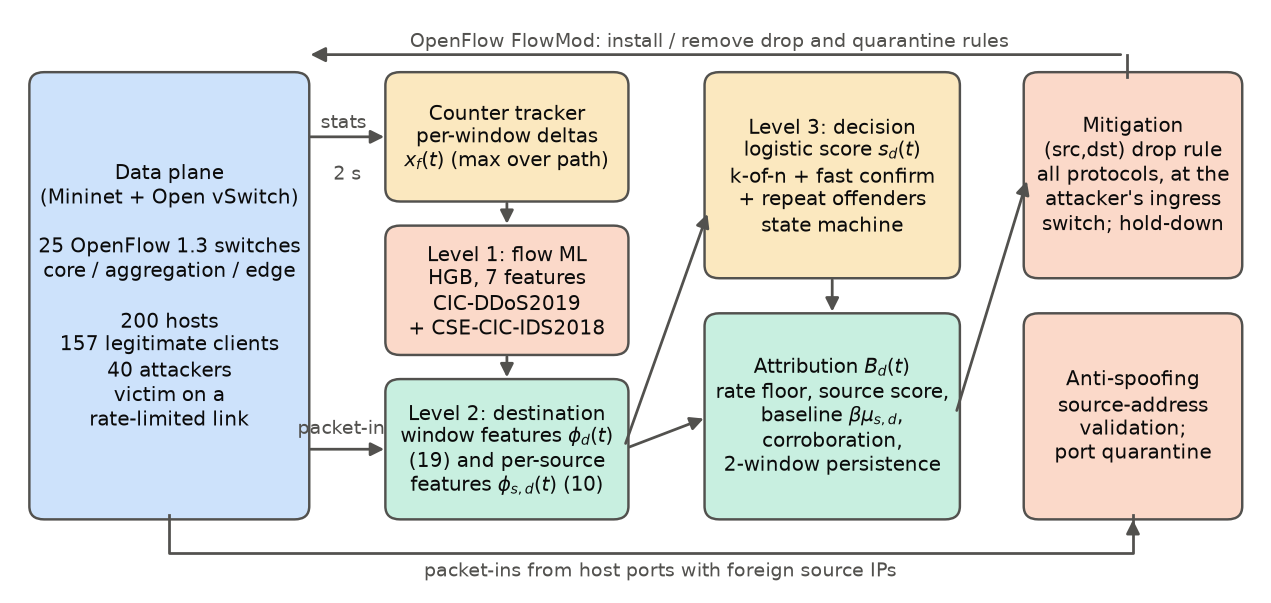
\includegraphics[width=0.82\textwidth]{fig_architecture.png}
\caption{Architecture: counter deltas feed a flow-level model (Level~1) and destination-centric window features (Level~2); a transparent decision layer (Level~3) confirms attacks, attributes sources and installs scoped OpenFlow rules.}
\label{fig:arch}
\end{figure*}

\subsection{Window score and confirmation}
The window score is a logistic model on transformed features,
\begin{equation}
s_d(t)=\sigma\big(w^\top\psi(\phi_d(t))+b\big),
\end{equation}
where $\psi$ applies $\log(1+x)$ to heavy-tailed features (counts and rates) and standardises with calibration statistics. A linear score was chosen deliberately: every alert is explained by the per-feature contributions $w_j\psi_j$, which the controller logs. A destination is confirmed when
\begin{multline}
\textstyle\sum_{i=0}^{n-1}\mathbb{1}\{s_d(t-i)\ge\eta\}\ge k\ \ \lor\ \ s_d(t)\ge\eta_f\\
\lor\ \ \big(s_d(t)\ge\eta\wedge R_d(t)\neq\emptyset\big),
\end{multline}
with $k$-of-$n$ $=2$-of-$3$, $\eta_f=0.97$, and $R_d(t)$ the sources blocked at $d$ within the last $M=300$\,s that are sending again (repeat offenders). A per-destination state machine (NORMAL, SUSPECTED, CONFIRMED, MITIGATING, RECOVERING) removes the rules of $d$ after $Q_e=Q\cdot2^{\min(e-1,3)}$ quiet windows in the $e$-th attack episode on $d$ ($Q=3$), i.e.\ with an exponential hold-down against pulsing attacks.

\subsection{Source attribution}
For a confirmed $d$ the block set is
\begin{multline}
B_d(t)=\big\{s:\ \lambda_{s,d}\ge\lambda_{\text{floor}}\ \wedge\ \lambda_{s,d}\ge\beta\,\mu_{s,d}\ \wedge\\
\big(r_{s,d}\ge\eta_s\ \lor\ (\lambda_{s,d}\ge\lambda_{\text{rate}}\wedge \mathrm{corr}(s))\big)\big\},
\end{multline}
where $r_{s,d}=\sigma(u^\top\psi(\phi_{s,d})+c)$ is a logistic source score, $\lambda_{\text{floor}}=15$\,pps, $\lambda_{\text{rate}}=150$\,pps, and $\mathrm{corr}(s)$ holds if the flow model flags $s$'s flows ($\max p_f\ge0.5$), if $s$ opens $\ge10$ new flows per window, or if $s$ was never seen sending to $d$ in normal windows. The baseline $\mu_{s,d}$ is a peak-hold average of $\lambda_{s,d}$ learned only in windows in which $d$ is NORMAL and below threshold ($\mu\leftarrow\max(\lambda,0.97\mu)$); with $\beta=3$ a source that already sent at that rate before the attack (a video stream, a bulk transfer) is not blocked unless its rate triples. Finally, a source enters $B_d$ only after qualifying in two consecutive windows (repeat offenders at once).

\subsection{Mitigation}
For each $s\in B_d$ one OpenFlow rule (priority 200, hard timeout 300\,s) matching \texttt{ipv4\_src}$=s$, \texttt{ipv4\_dst}$=d$ for \emph{all} IP protocols drops the traffic at $s$'s ingress switch, so switching from UDP to ICMP or TCP does not bypass it. For anti-spoofing, every host port $(\text{sw},p)$ is bound to its address $\beta(\text{sw},p)$; if a port emits $\ge\kappa=20$ packet-ins towards $d$ with a foreign source address in one window, a quarantine rule (\texttt{in\_port}$=p$, \texttt{ipv4\_dst}$=d$, drop) is installed on that switch. Algorithm~\ref{alg:main} summarises one polling cycle.

\begin{algorithm}[t]
\caption{One polling cycle of the controller}\label{alg:main}
\begin{algorithmic}[1]
\STATE Request flow statistics from all switches; wait $\le 1.5$\,s
\STATE Compute counter deltas $x_f(t)$ (max over path, re-installation aware)
\STATE Score active flows with $g_\theta$ (Level 1)
\STATE Build $\phi_d(t)$ for every destination, $\phi_{s,d}(t)$ for every pair
\FOR{each destination $d$}
  \STATE $s_d\gets\sigma(w^\top\psi(\phi_d)+b)$; update history
  \IF{state$_d\in\{$NORMAL$\}$ and $s_d<\eta$}
     \STATE update baselines $\mu_{s,d}$
  \ENDIF
  \IF{$k$-of-$n$ over $\eta$ \OR $s_d\ge\eta_f$ \OR ($s_d\ge\eta$ \AND $R_d\neq\emptyset$)}
     \STATE state$_d\gets$ CONFIRMED
  \ENDIF
  \IF{state$_d\in\{$CONFIRMED, MITIGATING$\}$ and $s_d\ge\eta$}
     \STATE compute $B_d$ (floor, baseline, score/corroboration, persistence)
     \STATE install one all-protocol drop rule per new $s\in B_d$ at its ingress switch
  \ENDIF
  \IF{quiet for $Q_e$ windows} \STATE remove the rules of $d$; state$_d\gets$ RECOVERING \ENDIF
\ENDFOR
\STATE Quarantine host ports with $\ge\kappa$ spoofed packet-ins per destination
\end{algorithmic}
\end{algorithm}

\subsection{Calibration}
The window and source models are fitted with class-balanced logistic regression ($C=1$) on a separate calibration session only. Their thresholds are the $(1-\varepsilon)$ quantile of leave-one-segment-out probabilities on benign windows, with $\varepsilon=0.3\,\%$ for the window model and $1\,\%$ for the source model (source decisions are only made at already confirmed victims). The baselines receive their thresholds the same way.

%=====================================================================
\section{Baselines and Experimental Setup}\label{sec:setup}
\subsection{Flow-level data}\label{sec:flowdata}
We map CIC-DDoS2019~\cite{sharafaldin2019ddos} (folder 01-12) and four days of CSE-CIC-IDS2018~\cite{sharafaldin2018toward} (15, 16, 21, 22 Feb.; DoS and DDoS classes kept, others dropped) to the seven features of Level~1 and remove all rows whose feature vectors are identical but whose labels differ. After cleaning, CIC-DDoS2019 has 1\,831\,822 flows with only 16\,733 benign (7\,302 benign UDP), and CSE-CIC-IDS2018 has 3\,654\,924 flows with 2\,557\,308 benign (647\,892 benign UDP). Splits are group-disjoint; each model is trained on 20\,000 flows per class per dataset and tested on natural-ratio holdouts of 60\,000 flows per dataset. Seven scikit-learn~\cite{pedregosa2011scikit} classifiers are compared; HistGradientBoosting follows the LightGBM design~\cite{ke2017lightgbm}.

\subsection{Testbed}
Mininet~\cite{lantz2010network} with Open vSwitch~\cite{pfaff2015ovs} (OpenFlow 1.3) emulates a three-tier tree: one core switch, four aggregation switches and 20 edge switches with 10 hosts each (25 switches, 200 hosts). Host links run at 100\,Mbit/s, edge--aggregation links at 200\,Mbit/s and aggregation--core links at 400\,Mbit/s. The victim h200 sits behind a 25\,Mbit/s access link in the test sessions (50\,Mbit/s in calibration). Two further servers carry only benign traffic. Forwarding entries are installed per (source, destination, protocol), the packet-in rate is limited to 400\,pps per switch, and flows idle out after 15\,s.

\textbf{Legitimate workload (157 clients).} 95 web clients (10\,kB/100\,kB pages, think time 0.5--3\,s, 60\,\% to the victim), 25 DNS-like UDP request/response clients (4 queries/s), 12 UDP video-like streams (1\,Mbit/s), 10 bulk TCP transfers (2\,Mbit/s) and 15 ping clients. About 17\,Mbit/s of benign load reaches the victim. Flash crowds make every web client fetch the large page six times in 20\,s.

\textbf{Attackers (40).} Two per edge switch, sharing switches with legitimate users, using hping3. Floods use 220--380\,pps per attacker (about 11\,000 pps offered), low-rate attacks 25--45\,pps, spoofed floods 120--180\,pps with random source addresses from four hosts.

\textbf{Sessions.} A calibration session (seed 1) and held-out sessions with seed 2 (new attacker subsets, rates and sizes). The test schedule is: benign, flash crowd, UDP, SYN, ICMP, low-rate, pulsing ($4\times$ 6\,s on / 10\,s off), spoofed, mixed UDP+SYN, protocol switching (UDP$\to$ICMP$\to$SYN, 20\,s each), re-attack (three 25\,s bursts 15\,s apart), benign, flash crowd, benign; attacks last 30--105\,s with 40\,s gaps. Two detection-only replicates (test\_det, test\_det2) give detection metrics; test\_det2 and a run with mitigation enabled (test\_mit) form a paired comparison. Ground truth (attacker addresses and intervals) comes from the scheduler, never from the detector. Every HTTP request, UDP query and ping reply of every client is logged (44\,000--56\,000 HTTP requests and 110\,000 UDP queries per session), and all edge-port counters are sampled every second.

\subsection{Baselines}
All baselines use the same features, the same 2-of-3 confirmation and thresholds set on calibration data at the same false-positive budget: (i) \emph{pps per destination} $\Lambda_d(t)>\eta_\Lambda$; (ii) \emph{source-IP entropy} of the packet distribution over sources at $d$ (bits); (iii) \emph{destination-IP entropy}~\cite{mousavi2015early}, the normalised entropy of all traffic over destinations, alarming on the dominant destination when it drops; (iv) \emph{flow-ML only}, $\max_f p_f$ at $d$.

%=====================================================================
\section{Results and Performance Analysis}\label{sec:results}
\subsection{Flow-level model}\label{sec:flow}
Fig.~\ref{fig:cross} shows that a model trained on one dataset does not transfer: HGB trained on CIC-DDoS2019 reaches a balanced accuracy of 0.998 on its own holdout but 0.421 on CSE-CIC-IDS2018, and vice versa 0.956 and 0.469. Training on both keeps 0.976 and 0.948. Table~\ref{tab:flow} compares all models trained on both datasets. HGB, Random Forest, Decision Tree and KNN are within 0.5 points; McNemar tests~\cite{mcnemar1947note,dietterich1998approximate} on the same 120\,000 test flows find RF ($-0.42$ points, $p=4\times10^{-18}$), KNN ($-0.26$, $p=7\times10^{-8}$) and DT ($-0.23$, $p=5\times10^{-6}$) slightly but significantly better than HGB. The differences are statistically detectable but not practically meaningful; we keep HGB because it is 4--5$\times$ faster than KNN, 23$\times$ smaller, and does not grow with the training set. The gains of the system come from Levels 2 and 3, not from the classifier.

\begin{figure}[t]
\centering
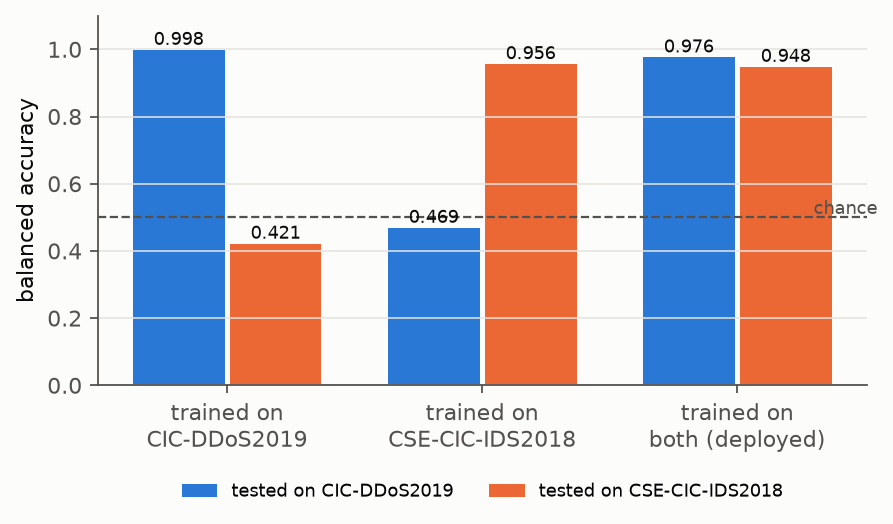
\includegraphics[width=\columnwidth]{fig_cross_dataset.png}
\caption{Balanced accuracy of HistGradientBoosting trained on one or both datasets and tested on each group-disjoint holdout.}
\label{fig:cross}
\end{figure}

\begin{table}[t]
\caption{Flow models trained on both datasets (balanced accuracy, false-positive rate, inference cost)}
\label{tab:flow}
\centering
\setlength{\tabcolsep}{3.5pt}
\begin{tabular}{lccccc}
\toprule
Model & BA'19 & FPR'19 & BA'18 & FPR'18 & $\mu$s/flow \\
\midrule
KNN & 0.982 & 2.8\,\% & 0.942 & 5.6\,\% & 15.6--20.0 \\
\textbf{HGB (used)} & \textbf{0.976} & \textbf{3.5\,\%} & \textbf{0.948} & \textbf{5.9\,\%} & \textbf{3.6--4.5} \\
Decision Tree & 0.972 & 4.4\,\% & 0.947 & 5.4\,\% & 0.2--0.3 \\
Random Forest & 0.971 & 4.6\,\% & 0.947 & 4.9\,\% & 5.6--6.1 \\
Extra Trees & 0.915 & 15.5\,\% & 0.903 & 12.7\,\% & 3.0--3.1 \\
Logistic Reg. & 0.666 & 37.4\,\% & 0.685 & 61.0\,\% & 0.3--0.5 \\
Naive Bayes & 0.594 & 1.8\,\% & 0.498 & 0.6\,\% & 0.3--0.4 \\
\bottomrule
\end{tabular}
\end{table}

\subsection{Detection on the large testbed}
Table~\ref{tab:detect} pools the two held-out detection sessions: 78\,141 destination windows (77\,755 benign, 386 under attack) and 18 attack episodes. Fig.~\ref{fig:methods} shows the window-level comparison for test\_det. The proposed detector has the highest recall (0.97) and F1 (0.78) at a 0.26\,\% window false-positive rate, and it is the only method that detects all 18 episodes; with the fast path its mean latency is 3.2\,s (4.5\,s without), compared with 5.4--7.7\,s for the baselines. Destination-IP entropy is a strong baseline in this setting (F1 0.74), because one victim receives a large share of all traffic, but it cannot identify sources and missed one spoofing episode. The rate threshold misses both low-rate episodes, source entropy misses both protocol-switching episodes, and the flow model alone misses the SYN floods (Table~\ref{tab:types}).

\begin{figure}[t]
\centering
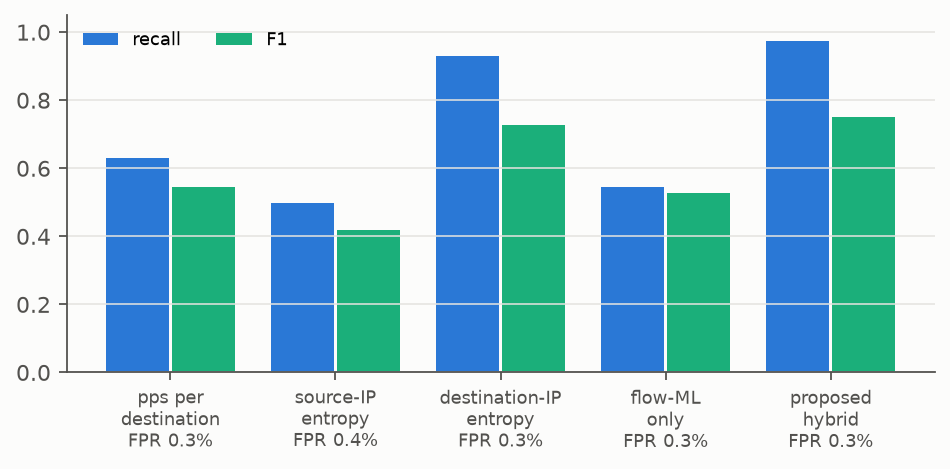
\includegraphics[width=\columnwidth]{fig_methods_large_test.png}
\caption{Window-level recall and F1 on the held-out session test\_det (same calibration false-positive budget for all methods).}
\label{fig:methods}
\end{figure}

\begin{table}[t]
\caption{Detection on two held-out 200-host sessions (pooled)}
\label{tab:detect}
\centering
\setlength{\tabcolsep}{2.6pt}
\begin{tabular}{lcccccc}
\toprule
Method & Rec. & FPR & F1 & Det. & Lat. & FA/h \\
\midrule
pps per destination & 0.63 & 0.35\,\% & 0.54 & 16/18 & 7.5\,s & 57 \\
Source-IP entropy & 0.56 & 0.45\,\% & 0.45 & 16/18 & 6.9\,s & 37 \\
Dest.-IP entropy~\cite{mousavi2015early} & 0.90 & 0.26\,\% & 0.74 & 17/18 & 5.4\,s & 30 \\
Flow-ML only & 0.56 & 0.24\,\% & 0.54 & 16/18 & 7.7\,s & 67 \\
Proposed (2-of-3) & 0.97 & 0.26\,\% & 0.78 & 18/18 & 4.5\,s & 40 \\
\textbf{Proposed + fast path} & \textbf{0.97} & \textbf{0.26\,\%} & \textbf{0.78} & \textbf{18/18} & \textbf{3.2\,s} & \textbf{45} \\
\bottomrule
\end{tabular}\\[2pt]
\footnotesize Rec./FPR/F1 per destination window; Det.: attack episodes detected; Lat.: mean detection latency; FA/h: false-alarm episodes per hour over all $\approx$100 active destinations.
\end{table}

\begin{table}[t]
\caption{Mean detection latency (s) per attack type over both sessions (--: not detected)}
\label{tab:types}
\centering
\setlength{\tabcolsep}{3pt}
\begin{tabular}{lccccc}
\toprule
Attack & Prop. & DstEnt & pps & SrcEnt & ML \\
\midrule
UDP flood & 3.7 & 5.7 & 1.7 & 1.7 & 5.7 \\
TCP SYN flood & 4.8 & 5.9 & 7.9 & 3.7 & -- \\
ICMP flood & 1.3 & 12.5 & 1.3 & 1.3 & 23.9 \\
Low-rate UDP & 5.1 & 1.1 & -- & 5.1 & 5.1 \\
Pulsing & 3.0 & 5.0 & 8.9 & 7.4 & 8.1 \\
Spoofed & 2.6 & 4.7$^\dagger$ & 2.6 & 2.6 & 4.8 \\
Mixed UDP+SYN & 1.2 & 5.4 & 23.7 & 24.7 & 6.6 \\
Protocol switching & 4.4 & 4.1 & 6.2 & -- & 5.3 \\
Re-attack & 2.4 & 3.7 & 7.7 & 8.7 & 2.4 \\
\midrule
Mean & \textbf{3.2} & 5.4 & 7.5 & 6.9 & 7.7 \\
\bottomrule
\end{tabular}\\[2pt]
\footnotesize $^\dagger$detected in one of the two sessions.
\end{table}

On the original 6-switch, 18-host chain testbed (21 held-out runs, 5\,s windows), the same comparison gives window F1 0.78 for the proposed detector against 0.42 (pps), 0.49 (source entropy), 0.47 (destination entropy) and 0.09 (flow-ML only), with 15 of 18 attack runs detected against at most 10.

\subsection{Mitigation and legitimate users}
Without protection, attacks hurt legitimate users through two channels. On the data plane the flood fills the 25\,Mbit/s link; during the UDP flood HTTP still succeeds but its 95th-percentile latency rises from 0.04\,s to 1.04\,s. On the control plane, at flood onset each attacker sends hundreds of packets before its forwarding entry exists; they fill the rate-limited packet-in queue, legitimate flows that need a new entry wait behind them, and from the ICMP flood onward legitimate service collapses and does not recover between attacks (Fig.~\ref{fig:pulse}). Table~\ref{tab:mitig} compares the paired sessions. Averaged over the nine attacks, legitimate HTTP success rises from 48\,\% to 89\,\%, DNS-like UDP success from 52\,\% to 94\,\%, ping delivery from 47\,\% to 86\,\% and bulk TCP throughput from 0.85 to 1.82\,Mbit/s (of 2.0 offered). Over the whole session 157 rules were installed, all 40 attackers were blocked at some time, four spoofing ports were quarantined 3.2\,s after onset, and \textbf{no legitimate host was blocked}. Repeat offenders were re-blocked 1.3\,s into a new burst, and protocol switching did not bypass the all-protocol rules. Fig.~\ref{fig:legit} shows HTTP success per attack.

\begin{figure}[t]
\centering
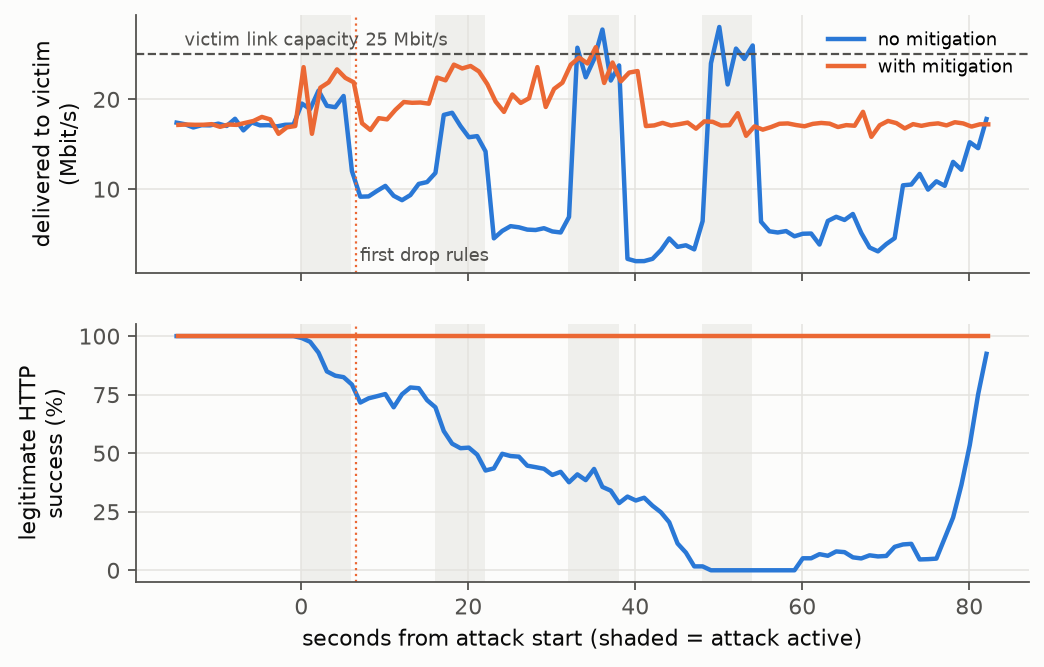
\includegraphics[width=\columnwidth]{fig_timeline_pulsing.png}
\caption{Pulsing attack (shaded bursts) on the same schedule without and with mitigation: delivered traffic at the victim and legitimate HTTP success (3\,s rolling mean).}
\label{fig:pulse}
\end{figure}

\begin{figure}[t]
\centering
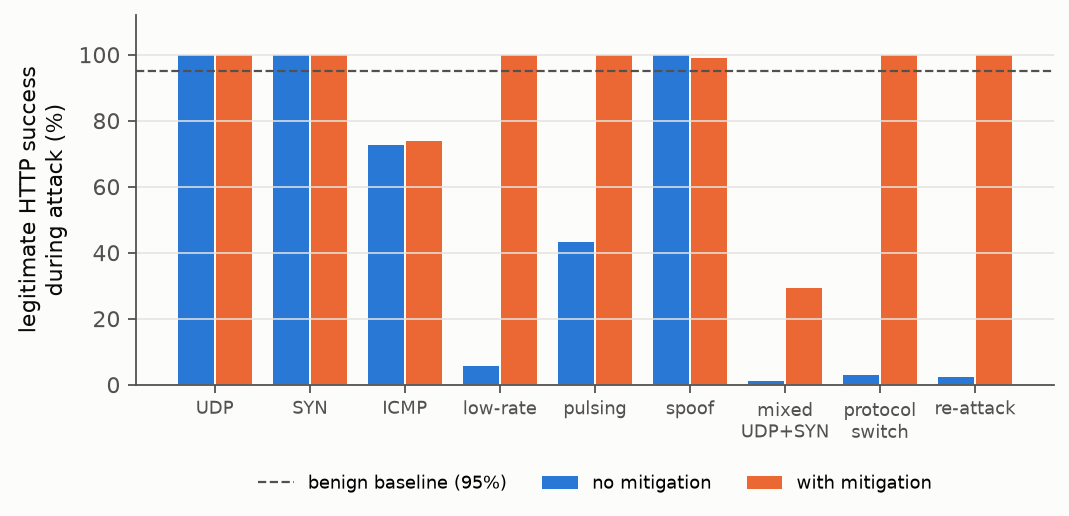
\includegraphics[width=\columnwidth]{fig_legit_http.png}
\caption{Legitimate HTTP success during each attack, paired sessions without and with mitigation.}
\label{fig:legit}
\end{figure}

\begin{table}[t]
\caption{Paired mitigation results (no mitigation $\to$ mitigation)}
\label{tab:mitig}
\centering
\setlength{\tabcolsep}{2.4pt}
\begin{tabular}{lccccc}
\toprule
Attack & 1st rule & Rules & HTTP & UDP query & Ping \\
\midrule
UDP flood & 9.9\,s & 38/40 & 1.00$\to$1.00$^*$ & 1.00$\to$1.00 & 0.99$\to$0.99 \\
TCP SYN & 6.8\,s & 36/40 & 1.00$\to$1.00 & 1.00$\to$1.00 & 0.98$\to$0.98 \\
ICMP & 3.7\,s & 1/40 & 0.73$\to$0.74 & 0.80$\to$0.79 & 0.16$\to$0.22 \\
Low-rate & -- & 0/40 & 0.06$\to$1.00 & 0.00$\to$1.00 & 0.34$\to$0.99 \\
Pulsing & 6.5\,s & 40/40 & 0.43$\to$1.00 & 0.69$\to$1.00 & 0.33$\to$0.99 \\
Spoofed & 3.2\,s & 4 ports & 1.00$\to$0.99 & 1.00$\to$1.00 & 0.98$\to$0.98 \\
Mixed & 3.7\,s & 34/40 & 0.01$\to$0.29 & 0.11$\to$0.66 & 0.02$\to$0.58 \\
Proto. switch & --$^\ddagger$ & 0/24 & 0.03$\to$1.00 & 0.00$\to$1.00 & 0.10$\to$0.98 \\
Re-attack & 1.3\,s & 4/30$^\ddagger$ & 0.02$\to$1.00 & 0.07$\to$1.00 & 0.28$\to$0.98 \\
\midrule
Mean & & & 0.48$\to$0.89 & 0.52$\to$0.94 & 0.47$\to$0.86 \\
\bottomrule
\end{tabular}\\[2pt]
\footnotesize Rules: new rules installed during the attack; 0 legitimate hosts blocked in every row. $^*$HTTP p95 latency 1.04\,s$\to$0.04\,s. $^\ddagger$Most bots still blocked from earlier episodes.
\end{table}

\subsection{Attribution ablation}\label{sec:ablation}
The final attribution rule was reached through three earlier mitigation runs on the same schedule (Table~\ref{tab:abl}). Without a per-source baseline, steady legitimate senders to the victim (video streams, bulk transfers) look like flood sources and nine were blocked. The baseline removed most of them; the remaining blocks were traced to one-window rate spikes caused by re-installed flow entries (e.g.\ a 104\,pps stream measured at 629\,pps), which the counter-delta correction and two-window persistence removed. Each change was validated offline by replaying a detection-only session before the next live run. Attacker coverage stayed at 97--98\,\% throughout.

\begin{table}[t]
\caption{Collateral blocking in successive mitigation runs}
\label{tab:abl}
\centering
\setlength{\tabcolsep}{3pt}
\begin{tabular}{llcc}
\toprule
Run & Attribution & Attackers & Legit blocked \\
\midrule
v1 & score + corroborated rate rule$^\S$ & 40 & 9 \\
v2 & + baseline $\beta\mu_{s,d}$ & 40 & 6 \\
v3 & + counter fix, new-source corr. & 40 & 5 \\
\textbf{final} & \textbf{+ 2-window persistence} & \textbf{40} & \textbf{0} \\
\bottomrule
\end{tabular}\\[2pt]
\footnotesize $^\S$stopped after 5 of 14 segments.
\end{table}

\subsection{Limitations}
ICMP floods are detected but their sources are not attributed live (1 of 40), although the same rule attributed 38 of 40 in an offline replay; mixed UDP+SYN floods only partly recover. Window precision (0.65) and 30--67 false-alarm episodes per hour across $\approx$100 destinations remain the main open problem for every method. All results come from one machine (8 cores, WSL2) with one calibration and two held-out sessions of the same seed; the attribution rules were refined while observing mitigation runs on the test schedule, so a fresh seed would be a cleaner confirmation. Traffic is scripted, not real user traces.

%=====================================================================
\section{Conclusion}
We formulated DDoS defence in SDN as quickest detection under a false-alarm budget combined with goodput-maximising, collateral-free block-set selection, and implemented a controller that solves a plug-in version of both problems. Destination-centric window features over a two-dataset flow model detect nine attack types on a 200-host network with F1 0.78 and 3.2\,s mean latency, better than standard rate and entropy baselines, and baseline-aware, persistence-filtered attribution with protocol-agnostic and anti-spoofing rules raises legitimate service during attacks from 48\,\% to 89\,\% without blocking any legitimate host. The experiments also show that the flow classifier is not where the gains come from, that single-dataset flow models do not transfer, and that the collateral constraint is the hard part of mitigation at scale. Future work is attribution for ICMP and mixed floods, fewer false alarms through per-destination adaptive thresholds, and validation on real traces and hardware switches.

%=====================================================================
\begin{thebibliography}{00}
\bibitem{mckeown2008openflow} N. McKeown \emph{et al.}, ``OpenFlow: Enabling innovation in campus networks,'' \emph{ACM SIGCOMM Comput. Commun. Rev.}, vol. 38, no. 2, pp. 69--74, 2008.
\bibitem{kreutz2015sdn} D. Kreutz, F. M. V. Ramos, P. E. Verissimo, C. E. Rothenberg, S. Azodolmolky, and S. Uhlig, ``Software-defined networking: A comprehensive survey,'' \emph{Proc. IEEE}, vol. 103, no. 1, pp. 14--76, 2015.
\bibitem{yan2016sdn} Q. Yan, F. R. Yu, Q. Gong, and J. Li, ``Software-defined networking (SDN) and distributed denial of service (DDoS) attacks in cloud computing environments: A survey, some research issues, and challenges,'' \emph{IEEE Commun. Surveys Tuts.}, vol. 18, no. 1, pp. 602--622, 2016.
\bibitem{shin2013avant} S. Shin, V. Yegneswaran, P. Porras, and G. Gu, ``AVANT-GUARD: Scalable and vigilant switch flow management in software-defined networks,'' in \emph{Proc. ACM CCS}, 2013, pp. 413--424.
\bibitem{wang2015floodguard} H. Wang, L. Xu, and G. Gu, ``FloodGuard: A DoS attack prevention extension in software-defined networks,'' in \emph{Proc. IEEE/IFIP DSN}, 2015, pp. 239--250.
\bibitem{sommer2010outside} R. Sommer and V. Paxson, ``Outside the closed world: On using machine learning for network intrusion detection,'' in \emph{Proc. IEEE Symp. Security and Privacy}, 2010, pp. 305--316.
\bibitem{braga2010lightweight} R. Braga, E. Mota, and A. Passito, ``Lightweight DDoS flooding attack detection using NOX/OpenFlow,'' in \emph{Proc. IEEE LCN}, 2010, pp. 408--415.
\bibitem{mousavi2015early} S. M. Mousavi and M. St-Hilaire, ``Early detection of DDoS attacks against SDN controllers,'' in \emph{Proc. Int. Conf. Computing, Networking and Communications (ICNC)}, 2015, pp. 77--81.
\bibitem{giotis2014combining} K. Giotis, C. Argyropoulos, G. Androulidakis, D. Kalogeras, and V. Maglaris, ``Combining OpenFlow and sFlow for an effective and scalable anomaly detection and mitigation mechanism on SDN environments,'' \emph{Comput. Netw.}, vol. 62, pp. 122--136, 2014.
\bibitem{bawany2017ddos} N. Z. Bawany, J. A. Shamsi, and K. Salah, ``DDoS attack detection and mitigation using SDN: Methods, practices, and solutions,'' \emph{Arabian J. Sci. Eng.}, vol. 42, no. 2, pp. 425--441, 2017.
\bibitem{tang2016deep} T. A. Tang, L. Mhamdi, D. McLernon, S. A. R. Zaidi, and M. Ghogho, ``Deep learning approach for network intrusion detection in software defined networking,'' in \emph{Proc. Int. Conf. Wireless Networks and Mobile Communications (WINCOM)}, 2016, pp. 258--263.
\bibitem{niyaz2017deep} Q. Niyaz, W. Sun, and A. Y. Javaid, ``A deep learning based DDoS detection system in software-defined networking (SDN),'' \emph{EAI Endorsed Trans. Security and Safety}, vol. 4, no. 12, 2017.
\bibitem{sharafaldin2019ddos} I. Sharafaldin, A. H. Lashkari, S. Hakak, and A. A. Ghorbani, ``Developing realistic distributed denial of service (DDoS) attack dataset and taxonomy,'' in \emph{Proc. IEEE Int. Carnahan Conf. Security Technology (ICCST)}, 2019, pp. 1--8.
\bibitem{sharafaldin2018toward} I. Sharafaldin, A. H. Lashkari, and A. A. Ghorbani, ``Toward generating a new intrusion detection dataset and intrusion traffic characterization,'' in \emph{Proc. Int. Conf. Information Systems Security and Privacy (ICISSP)}, 2018, pp. 108--116.
\bibitem{rfc2827} P. Ferguson and D. Senie, ``Network ingress filtering: Defeating denial of service attacks which employ IP source address spoofing,'' IETF RFC 2827 (BCP 38), 2000.
\bibitem{rfc7039} J. Wu, J. Bi, M. Bagnulo, F. Baker, and C. Vogt, ``Source Address Validation Improvement (SAVI) framework,'' IETF RFC 7039, 2013.
\bibitem{page1954continuous} E. S. Page, ``Continuous inspection schemes,'' \emph{Biometrika}, vol. 41, no. 1/2, pp. 100--115, 1954.
\bibitem{lorden1971procedures} G. Lorden, ``Procedures for reacting to a change in distribution,'' \emph{Ann. Math. Statist.}, vol. 42, no. 6, pp. 1897--1908, 1971.
\bibitem{kuzmanovic2003low} A. Kuzmanovic and E. W. Knightly, ``Low-rate TCP-targeted denial of service attacks: The shrew vs. the mice and elephants,'' in \emph{Proc. ACM SIGCOMM}, 2003, pp. 75--86.
\bibitem{jung2002flash} J. Jung, B. Krishnamurthy, and M. Rabinovich, ``Flash crowds and denial of service attacks: Characterization and implications for CDNs and web sites,'' in \emph{Proc. WWW}, 2002, pp. 293--304.
\bibitem{ryu} Ryu SDN Framework Community, ``Ryu: Component-based software defined networking framework.'' [Online]. Available: https://ryu-sdn.org
\bibitem{pedregosa2011scikit} F. Pedregosa \emph{et al.}, ``Scikit-learn: Machine learning in Python,'' \emph{J. Mach. Learn. Res.}, vol. 12, pp. 2825--2830, 2011.
\bibitem{ke2017lightgbm} G. Ke \emph{et al.}, ``LightGBM: A highly efficient gradient boosting decision tree,'' in \emph{Proc. NeurIPS}, 2017, pp. 3146--3154.
\bibitem{lantz2010network} B. Lantz, B. Heller, and N. McKeown, ``A network in a laptop: Rapid prototyping for software-defined networks,'' in \emph{Proc. ACM HotNets}, 2010, pp. 1--6.
\bibitem{pfaff2015ovs} B. Pfaff \emph{et al.}, ``The design and implementation of Open vSwitch,'' in \emph{Proc. USENIX NSDI}, 2015, pp. 117--130.
\bibitem{mcnemar1947note} Q. McNemar, ``Note on the sampling error of the difference between correlated proportions or percentages,'' \emph{Psychometrika}, vol. 12, no. 2, pp. 153--157, 1947.
\bibitem{dietterich1998approximate} T. G. Dietterich, ``Approximate statistical tests for comparing supervised classification learning algorithms,'' \emph{Neural Comput.}, vol. 10, no. 7, pp. 1895--1923, 1998.
\end{thebibliography}

\end{document}
